 \documentclass[a4paper,11pt]{article}
 \usepackage{latexsym}
 \usepackage[utf8]{inputenc}
 \usepackage[activeacute,spanish]{babel}
 \RequirePackage{graphicx}
 \RequirePackage{booktabs}
 \title{REPORTE: ESTIMACIÓN DE PARÁMETROS DE TSUNAMI DE ORIGEN LEJANO}
 \author{Cesar Jimenez \\
 (Version: 1.1)}
 \frenchspacing
 \begin{document}
 \renewcommand{\tablename}{Tabla}
 \maketitle
 \section*{Introducción}
 \noindent
 Este reporte preliminar de tsunami de origen lejano ha sido 
 elaborado en forma automática por el modelo numérico TSDHN-2022.
 Las dimensiones de la fuente sísmica se calculan a partir de las ecuaciones de
  Papazachos et al. (2004).
 El mecanismo focal del terremoto se toma de la base de datos del Global CMT.
 El campo de deformación se obtiene a partir de las ecuaciones analíticas de O
 kada (1992).
  
 La simulación de la propagación del tsunami se realiza con el modelo numéric
 o TUNAMI,
 modelo lineal y en coordenadas esféricas (Imamura et al., 2006).
 La grilla batimétrica computacional abarca todo el Océano Pacífico, con una 
 resolución de 4 min o 240 seg.
 El tiempo promedio de cómputo para una PC i7 es de 20 min para una ventana de 
 tiempo de simulación
 de 28 horas (Figura 1). Sin embargo, el supercomputador DHN demora menos de 2 m
 inutos.
  
 \textbf{Nota:} El resultado del modelo TSDHN-2022 es una estimacion referencial
  y solo debe ser utilizado para
 obtener los parámetros de tsunamis de origen lejano, es decir fuera de las fro
 nteras del litoral de Perú.
 Para eventos de origen cercano, se debe utilizar el modelo Pre-Tsunami (Jimenez
  et al., 2018).
 \section*{Análisis}
 La Tabla 1 muestra los parámetros hipocentrales y el mecanismo focal del terre
 moto
 La Figura 1 muestra el mapa de propagacion de la máxima energía, la ubicació
 n del epicentro está representado
 por la esfera focal y las estaciones mareográficas están representadas por lo
 s triángulos azules
  
 La Figura 2 muestra los mareogramas simulados para las estaciones del litoral d
 el Perú,
 de norte a sur: Talara, Callao y Matarani
 La Tabla 2 muestra los tiempos de arribo y la máxima altura del tsunami
 en las estaciones mareográficas del litoral peruano.
 \begin{table*}
 \centerline{
 \begin{tabular}[t]{lp{0.5cm}l}
 \toprule
 Parámetro   & & Valor \\
 \midrule
Latitud     & &    0.95$^\circ$  \\
Longitud    & &  -79.37$^\circ$  \\
Profundidad & &   20.0 km       \\
Magnitud    & &    8.8 Mw       \\
 \midrule
Strike      & &   27.0$^\circ$  \\
Dip         & &   15.0$^\circ$  \\
Rake        & &   90.0$^\circ$  \\
 \bottomrule
 \end{tabular}}
 \caption{Parámetros hipocentrales y mecanismo focal del terremoto.}
 \end{table*}
 \begin{figure}
 \centerline{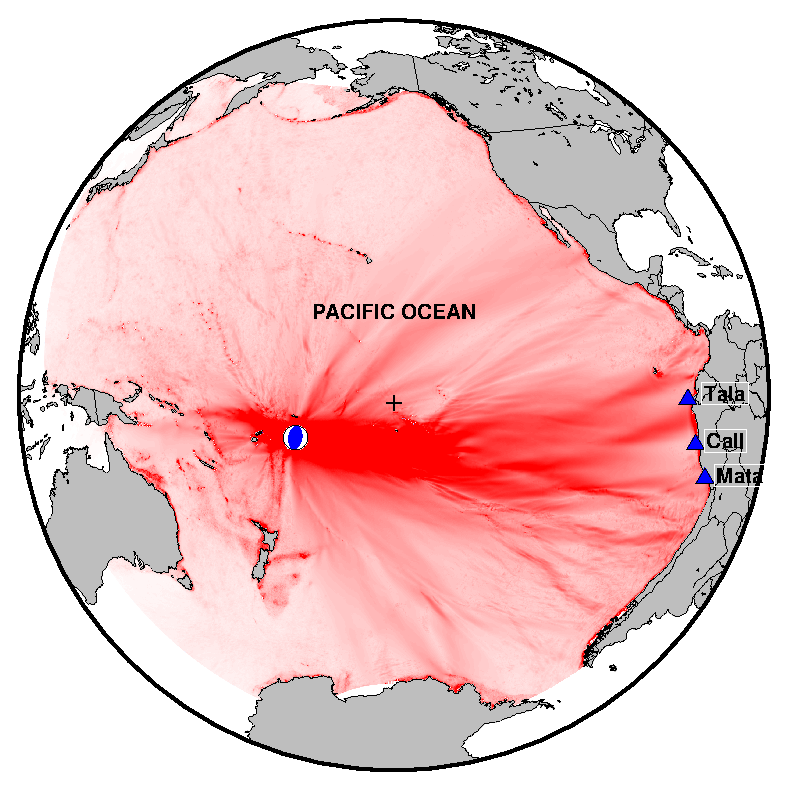
\includegraphics[scale=0.88]{maxola.eps}}
 \caption{Mapa de máxima altura de propagación del tsunami. La esfera focal re
 presenta el epicentro.
 Los triángulos azules representan a las estaciones mareográficas.}
 \label{mareograma}
 \end{figure}
 \begin{figure}
 \centerline{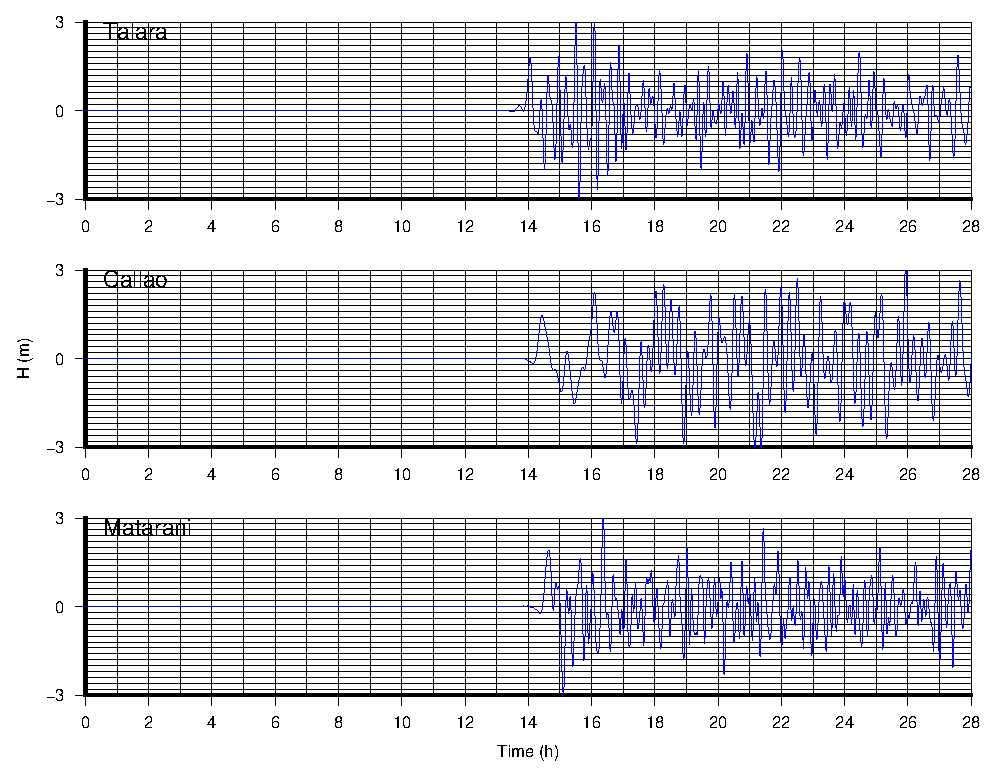
\includegraphics[scale=0.84]{mareograma.eps}}
 \caption{Mareogramas simulados en las estaciones de Talara, Callao y Matarani.}
 \end{figure}
 \begin{table*}
 \centerline{
 \begin{tabular}[t]{lcc}
 \toprule
 Estación     & Tiempo de arribo & Máximo (m) \\
 \midrule
Talara     & 0:27 &   0.62  \\
Callao     & 2:45 &   0.47  \\
Matarani   & 3:36 &   0.21  \\
 \bottomrule
 \end{tabular}}
 \caption{Tiempo de arribo (hh:mm) y máxima amplitud del tsunami.}
 \end{table*}
 \begin{thebibliography}{99}
 \bibitem{1} B. Papazachos, E. Scordilis, C. Panagiotopoulus and G. Karakaisis. 
 Global relations between seismic
 fault parameters and moment magnitude of earthquakes. Bulletin of Geological So
 ciety of Greece,
 vol XXXVI, pp 1482-1489 (2004).
 \bibitem{2} Y. Okada. Internal deformation in a half space. Bull. Seismol. Soc.
 Am. {82}(2) 1018-1040 (1992).
 \bibitem{3} F. Imamura, A. Yalciner and G. Ozyurt. Tsunami Modelling Manual
 (TUNAMI model). Tohoku University, Sendai. (2006).
 \bibitem{4} C. Jiménez, C. Carbonel and J. Rojas. Numerical procedure to forec
 ast the tsunami parameters from a
 database of pre-simulated seismic unit sources. Pure Appl. Geophys., vol 175, p
 p 1473--1483 (2018).
 \end{thebibliography}
 \end{document}
